% !TEX program = pdflatex
% !TEX options = -shell-escape -synctex=1 -interaction=nonstopmode -file-line-error "%DOC%"
%\documentclass[multi={mymath},border=2,crop]{standalone}
\documentclass{article}
\usepackage{amsmath}
\usepackage{amssymb}
\usepackage{amsfonts}
\usepackage{tikz}
\usetikzlibrary{matrix,arrows,calc,through,external}
\tikzexternalize[prefix=tikz/, figure name=constructible]
\usepackage{tikz-cd} % despite we don't explicitly used tikzcd, it is necessary because it loads some TiKZ libraries necessary to type tikzcd-like tikzpictures
\usepackage{ifthen}
\usepackage{enumitem}
\usepackage{graphicx}

\begin{document}


\tikzsetnextfilename{jordanblock}

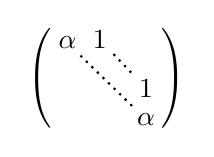
\begin{tikzpicture}
\matrix (m) [matrix of math nodes, row sep=5, column sep=5,left delimiter={(},right delimiter={)}, inner sep=.5]
{
	\alpha&1&&\\
	&&&\\
	&&&1\\
	&&&\alpha\\
};
\draw[dotted, thick, shorten <= 2.5pt, shorten <= 2.5pt, shorten >= 2.5pt] (m-1-1) -- (m-4-4);
\draw[dotted, thick, shorten <= 2.5pt, shorten <= 2.5pt, shorten >= 2.5pt] (m-1-2) -- (m-3-4);
\end{tikzpicture}


\tikzsetnextfilename{jordanmatrix}

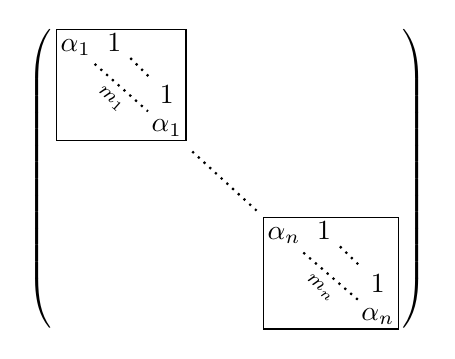
\begin{tikzpicture}
\matrix (m) 
[matrix of math nodes, 
row sep=5, 
column sep=5,
left delimiter={(},
right delimiter={)}, 
inner sep=.5,
outer sep=1]
{
	\alpha_1&1&&\\
	&&&\\
	&&&1\\
	&&&\alpha_1\\
	&&&&\\
	&&&&&\\
	&&&&&&\\
	&&&&&&&\\
	&&&&&&&&\\
	&&&&&&&&&\alpha_n&1\\
	&&&&&&&&&&\\
	&&&&&&&&&&&&1\\
	&&&&&&&&&&&&\alpha_n\\
};
\draw[dotted, thick, shorten <= 2.5pt, shorten >= 2.5pt] (m-1-1) -- (m-4-4) node [sloped, midway, below] {$\scriptstyle m_1$};
\draw[dotted, thick, shorten <= 2.5pt, shorten >= 2.5pt] (m-1-2) -- (m-3-4);
\draw (m-1-1.west|-m-1-2.north) rectangle (m-4-4.south east);
\draw[dotted, thick, shorten <= 6pt, shorten >= 7pt] (m-4-4) -- (m-10-10);
\draw[dotted, thick, shorten <= 2.5pt, shorten >= 2.5pt] (m-10-10) -- (m-13-13) node [sloped, midway, below] {$\scriptstyle m_n$};
\draw[dotted, thick, shorten <= 2.5pt, shorten >= 2.5pt] (m-10-11) -- (m-12-13);
\draw (m-10-10.west|-m-10-11.north) rectangle (m-13-13.south east);
\end{tikzpicture}



\tikzsetnextfilename{fractionfield}

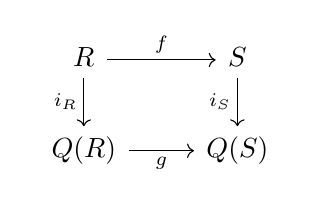
\begin{tikzpicture}[commutative diagrams/every diagram]
	\matrix[matrix of math nodes, name=m, commutative diagrams/every cell] {
	R & 
	S \\
	Q(R) &
	Q(S) \\ };
	\path[commutative diagrams/.cd, every arrow, every label]
	(m-1-1) edge node {$f$} (m-1-2) 
			edge node [swap] {$i_R$} (m-2-1) 
	(m-2-1) edge node [swap] {$g$} (m-2-2)
	(m-1-2) edge node [swap] {$i_S$} (m-2-2);
\end{tikzpicture}


\tikzsetnextfilename{isomorfiamodulos}

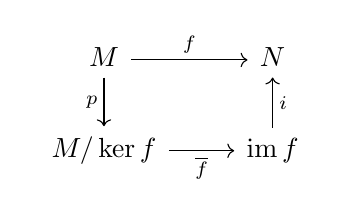
\begin{tikzpicture}[commutative diagrams/every diagram]
	\matrix[matrix of math nodes, name=m, commutative diagrams/every cell] {
	M & 
	N \\
	M/\ker f &
	\operatorname{im} f \\ };
	\path[commutative diagrams/.cd, every arrow, every label]
	(m-1-1) edge node {$f$} (m-1-2) 
			edge node [swap] {$p$} (m-2-1) 
	(m-2-1) edge node [swap] {$\overline{f}$} (m-2-2)
	(m-2-2) edge node [swap] {$i$} (m-1-2);
\end{tikzpicture}


\tikzsetnextfilename{isomorfianillos}

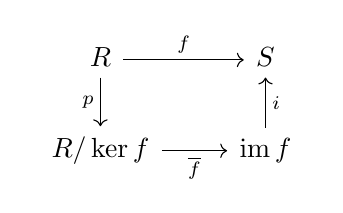
\begin{tikzpicture}[commutative diagrams/every diagram]
	\matrix[matrix of math nodes, name=m, commutative diagrams/every cell] {
	R & 
	S \\
	R/\ker f &
	\operatorname{im} f \\ };
	\path[commutative diagrams/.cd, every arrow, every label]
	(m-1-1) edge node {$f$} (m-1-2) 
			edge node [swap] {$p$} (m-2-1) 
	(m-2-1) edge node [swap] {$\overline{f}$} (m-2-2)
	(m-2-2) edge node [swap] {$i$} (m-1-2);
\end{tikzpicture}


\tikzsetnextfilename{libres}

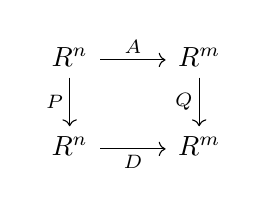
\begin{tikzpicture}[commutative diagrams/every diagram]
	\matrix[matrix of math nodes, name=m, commutative diagrams/every cell] {
	R^n & 
	R^m \\
	R^n &
	R^m \\ };
	\path[commutative diagrams/.cd, every arrow, every label]
	(m-1-1) edge node {$A$} (m-1-2) 
			edge node [swap] {$P$} (m-2-1) 
	(m-2-1) edge node [swap] {$D$} (m-2-2)
	(m-1-2) edge node [swap] {$Q$} (m-2-2);
\end{tikzpicture}


\tikzsetnextfilename{puntos}

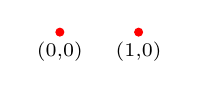
\begin{tikzpicture}
	\tikzstyle{bullet} = [circle, fill, draw, inner sep=1pt, red]
	\coordinate (A) at (0,0);
	\coordinate (B) at (1,0);
	\node[bullet] at (A) {}; 
	\node at (A) [below] {$\scriptstyle (0,0)$};
	\node[bullet] at (B) {}; 
	\node at (B) [below] {$\scriptstyle (1,0)$};
\end{tikzpicture}


\tikzsetnextfilename{recta}

\begin{tikzpicture}
	\path [use as bounding box] (-1,-1) rectangle (3,1.5);
	\tikzstyle{every node} = [circle, fill, draw, inner sep=1pt]
	\coordinate (A) at (0,0);
	\coordinate (B) at (2,1);
	\node at (A) {}; 
	\node at (B) {}; 
	\draw[shorten >= -.5cm, shorten <=-.8cm, red, thick] (A) -- (B);
\end{tikzpicture}


\tikzsetnextfilename{circunferencia}

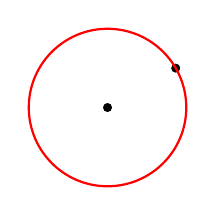
\begin{tikzpicture}
	\tikzstyle{every node} = [circle, fill, draw, inner sep=1pt]
	\coordinate (A) at (0,0);
	\coordinate (B) at (30:1cm);
	\node at (A) {}; 
	\node at (B) {}; 
	\draw[red, thick] (A) circle (1cm);
\end{tikzpicture}


\tikzsetnextfilename{intersec_rectas}

\begin{tikzpicture}
	\path [use as bounding box] (-1,-1) rectangle (1,1);
	\coordinate (A) at (0,0);
	\coordinate (B) at (-1,-.3);
	\coordinate (C) at (.2,-1);
	\draw[shorten >= -.5cm, shorten <=-.8cm] (A) -- (B);
	\draw[shorten >= -.5cm, shorten <=-.8cm] (A) -- (C);
	\node[circle, fill, draw, inner sep=1pt, red] at (A) {};
\end{tikzpicture}


\tikzsetnextfilename{intersec_recta_circ}

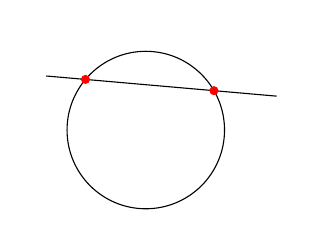
\begin{tikzpicture}
	\path [use as bounding box] (-1.5,-1) rectangle (2,1.3);
	\tikzstyle{every node} = [circle, fill, draw, inner sep=1pt, red]
	\coordinate (A) at (0,0);
	\coordinate (B) at (30:1cm);
	\coordinate (C) at (140:1cm);
	\draw (A) circle (1cm);
	\draw[shorten >= -.5cm, shorten <=-.8cm] (B) -- (C);
	\node at (B) {}; 
	\node at (C) {}; 
\end{tikzpicture}


\tikzsetnextfilename{intersec_circs}

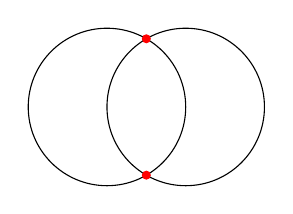
\begin{tikzpicture}
	\tikzstyle{every node} = [circle, fill, draw, inner sep=1pt, red]
	\coordinate (A) at (0,0);
	\coordinate (B) at (1,0);
	\coordinate (C) at (60:1cm);
	\coordinate (D) at (-60:1cm);
	\draw (A) circle (1cm);
	\draw (B) circle (1cm);
	\node at (C) {}; 
	\node at (D) {}; 
\end{tikzpicture}


\tikzsetnextfilename{medio}

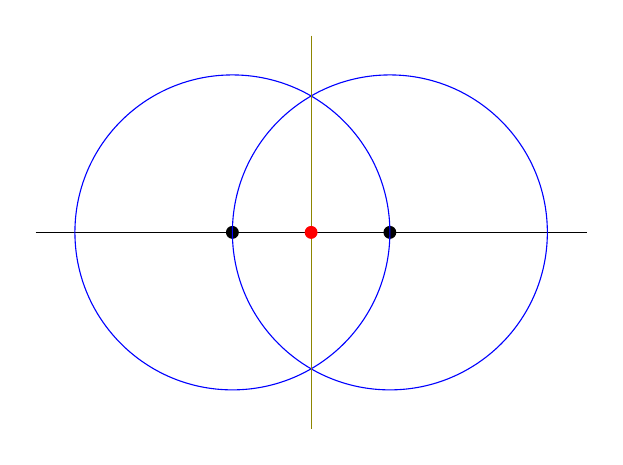
\begin{tikzpicture}[scale=2]
\path [use as bounding box] (-1.8,-1.3) rectangle (1.8,1.3);
\tikzstyle{every node} = [circle, fill, draw, inner sep=1.5pt]
\coordinate (A) at (-.5,0);
\coordinate (B) at (.5,0);
\coordinate (C) at (0,0);
\draw[shorten >= -2.5cm, shorten <= -2.5cm] (A) -- (B);	
\node at (A) {};
\node at (B) {};
\node[circle through=(A), fill=none, blue] at (B)  {};
\node[circle through=(B), fill=none, blue] at (A)  {};
\draw[shorten >= -2.5cm, shorten <= -.5cm, olive] (0,1) -- (C);	
\node[red] at (C) {};
\end{tikzpicture}


\tikzsetnextfilename{perpendicular_exterior}

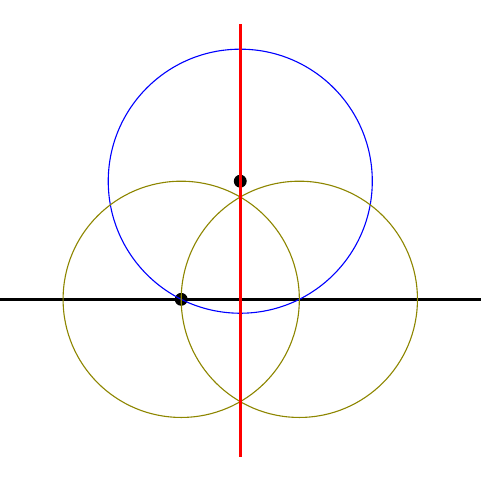
\begin{tikzpicture}[scale=1.5]
	\path [use as bounding box] (-1.8,-1.3) rectangle (1.8,2.3);
	\tikzstyle{every node} = [circle, fill, draw, inner sep=1.5pt]
	\coordinate (A) at (-.5,0);
	\coordinate (B) at (.5,0);
	\coordinate (C) at (0,1);
	\draw[shorten >= -2.5cm, shorten <= -2.5cm, very thick] (A) -- (B);	
	\node at (A) {};
	\node at (C) {}; 
	\node[circle through=(A), fill=none, blue] at (C)  {};
	\node[circle through=(A), fill=none, olive] at (B)  {};
	\node[circle through=(B), fill=none, olive] at (A)  {};
	\draw[shorten >= -2cm, shorten <= -2cm, red, very thick] (0,0) -- (C);	
\end{tikzpicture}


\tikzsetnextfilename{perpendicular_interior}

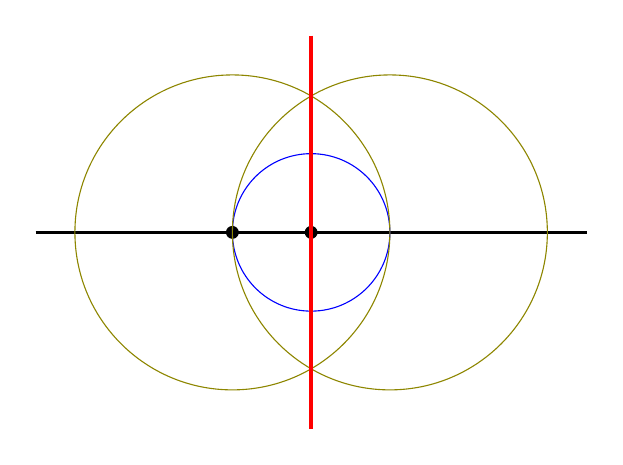
\begin{tikzpicture}[scale=2]
	\path [use as bounding box] (-1.8,-1.3) rectangle (1.8,1.3);
	\tikzstyle{every node} = [circle, fill, draw, inner sep=1.5pt]
	\coordinate (A) at (-.5,0);
	\coordinate (B) at (.5,0);
	\coordinate (C) at (0,0);
	\draw[shorten >= -2.5cm, shorten <= -2.5cm, very thick] (A) -- (B);	
	\node at (A) {};
	\node at (C) {}; 
	\node[circle through=(A), fill=none, blue] at (C)  {};
	\node[circle through=(A), fill=none, olive] at (B)  {};
	\node[circle through=(B), fill=none, olive] at (A)  {};
	\draw[shorten >= -2.5cm, shorten <= -.5cm, red, very thick] (0,1) -- (C);	
\end{tikzpicture}


\tikzsetnextfilename{paralela}

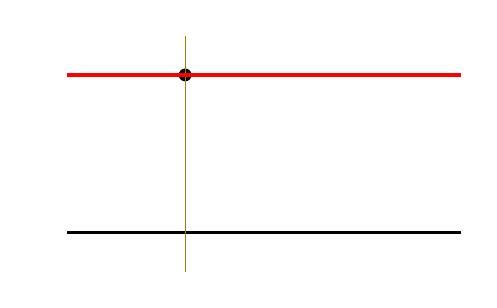
\begin{tikzpicture}[scale=2]
\path [use as bounding box] (-1,-.3) rectangle (1.8,1.3);
\tikzstyle{every node} = [circle, fill, draw, inner sep=1.5pt]
\coordinate (A) at (0,0);
\coordinate (B) at (1,0);
\coordinate (C) at (0,1);
\coordinate (D) at (1,1);
\draw[shorten >= -1.5cm, shorten <= -1.5cm, very thick] (A) -- (B);	
\node at (C) {}; 
\draw[shorten >= -.5cm, shorten <= -.5cm, olive] (A) -- (C);	
\draw[shorten >= -1.5cm, shorten <= -1.5cm, red, very thick] (C) -- (D);
\end{tikzpicture}


\tikzsetnextfilename{distancia}

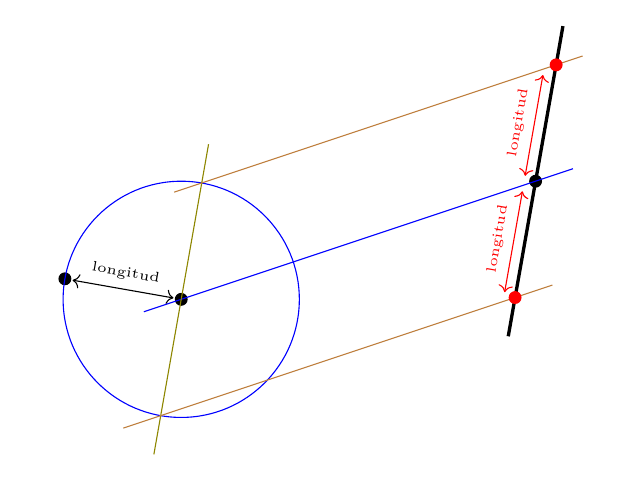
\begin{tikzpicture}[scale = 1.5]
\path [use as bounding box] (-1.3,-1.3) rectangle (3.5,2.3);
\tikzstyle{bullet} = [circle, fill, draw, inner sep=1.5pt]
\coordinate (A) at (0,0);
\coordinate (B) at (170:1cm);
\coordinate (C) at (3,1);
\node[bullet] at (A) {};
\node[bullet] at (B) {}; 
\node[bullet] at (C) {};
	\draw[<->, shorten >= .1cm, shorten <= .1cm] (A) -- node [above, sloped] {\tiny longitud} (B); 
	\draw[shorten >= -.5cm, shorten <= -2cm, very thick] (C) -- +(80:1cm) node (D) {};
	\draw[shorten >= -.5cm, shorten <= -.5cm, blue] (A) -- (C);
	\draw[blue] (A) circle (1cm);
	\draw[shorten >= -.5cm, shorten <= -2cm, olive] (A) -- +(80:1cm) node (E) {};
	\draw[shorten >= -.5cm, shorten <= -.5cm, brown] (D) -- (E);
	\draw[shorten >= -.5cm, shorten <= -.5cm, brown] ($(C)+(C)-(D)$) node (DD) {} -- ($(A)+(A)-(E)$) node (EE) {};
	\draw[<->, shorten >= .1cm, shorten <= .1cm, red] ($(C)+(-.1,-.02)$) -- node [above, sloped] {\tiny longitud} +(80:1cm); 
	\draw[<->, shorten >= .1cm, shorten <= .1cm, red] ($(C)+(-.1,-.02)$) -- node [above, sloped] {\tiny longitud} +(-100:1cm); 
	\node[bullet, red] at (D) {};
	\node[bullet, red] at (DD) {};
\end{tikzpicture}


\tikzsetnextfilename{coordenadas}

\begin{tikzpicture}[scale=1.5]
	\tikzstyle{bullet} = [circle, fill, draw, inner sep=1.5pt]
	\draw (-1,0) -- (3,0);
	\draw (0,-1) -- (0,2);
	\coordinate (O) at (0,0);
	\coordinate (P) at (2,1);
	\coordinate (A) at (2,0);
	\coordinate (B) at (0,1);
	\node[above right] at (P)  {$\scriptstyle (a,b)$};
	\draw[shorten >= -.5cm, shorten <= -.5cm, blue] (P) -- (A);
	\draw[shorten >= -.5cm, shorten <= -.5cm, blue] (P) -- (B);
	\draw[<->,shorten >= .1cm, shorten <= .1cm, purple] ($(O)+(0,-.1)$) -- node [below] {$\scriptstyle |a|$} ($(A)+(0,-.1)$);
	\draw[<->,shorten >= .1cm, shorten <= .1cm, purple] ($(O)+(-.1,0)$) -- node [left] {$\scriptstyle |b|$} ($(B)+(-.1,0)$);
	\node[bullet] at (O) {}; 
	\node[bullet, blue] at (P) {}; 
	\node[bullet, purple] at (A) {};
	\node[bullet, purple] at (B) {};
\end{tikzpicture}


\tikzsetnextfilename{suma}

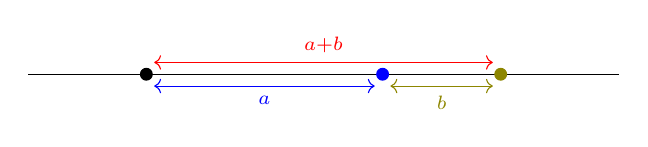
\begin{tikzpicture}[scale=1.5]
\tikzstyle{bullet} = [circle, fill, draw, inner sep=1.5pt]
\draw (-1,0) -- (4,0);
\coordinate (O) at (0,0);
\coordinate (A) at (2,0);
\coordinate (B) at (3,0);
\node[bullet] at (O) {}; 
\node[bullet, blue] at (A) {}; 
\node[bullet, olive] at (B) {};
\draw[<->,shorten >= .1cm, shorten <= .1cm, blue] ($(O)+(0,-.1)$) -- node [below] {$\scriptstyle a$} ($(A)+(0,-.1)$);
\draw[<->,shorten >= .1cm, shorten <= .1cm, olive] ($(A)+(0,-.1)$) -- node [below] {$\scriptstyle b$} ($(B)+(0,-.1)$);
\draw[<->,shorten >= .1cm, shorten <= .1cm, red] ($(O)+(0,.1)$) -- node [above] {$\scriptstyle a+b$} ($(B)+(0,.1)$);
\end{tikzpicture}


\tikzsetnextfilename{resta}

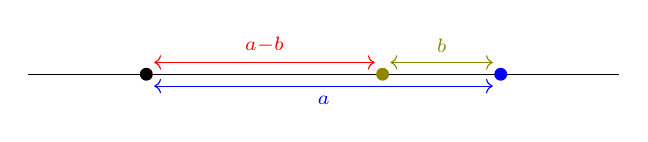
\begin{tikzpicture}[scale=1.5]
\tikzstyle{bullet} = [circle, fill, draw, inner sep=1.5pt]
\draw (-1,0) -- (4,0);
\coordinate (O) at (0,0);
\coordinate (B) at (2,0);
\coordinate (A) at (3,0);
\node[bullet] at (O) {}; 
\node[bullet, blue] at (A) {}; 
\node[bullet, olive] at (B) {};
\draw[<->,shorten >= .1cm, shorten <= .1cm, blue] ($(O)+(0,-.1)$) -- node [below] {$\scriptstyle a$} ($(A)+(0,-.1)$);
\draw[<->,shorten >= .1cm, shorten <= .1cm, olive] ($(A)+(0,.1)$) -- node [above] {$\scriptstyle b$} ($(B)+(0,.1)$);
\draw[<->,shorten >= .1cm, shorten <= .1cm, red] ($(O)+(0,.1)$) -- node [above] {$\scriptstyle a-b$} ($(B)+(0,.1)$);
\end{tikzpicture}


\tikzsetnextfilename{producto}

\begin{tikzpicture}[scale=1.5]
	\path [use as bounding box] (-1,-1) rectangle (4,2);
	\tikzstyle{bullet} = [circle, fill, draw, inner sep=1.5pt]
	\draw (-1,0) -- (4,0);
	\coordinate (O) at (0,0);
	\coordinate (U) at (2,0);
	\coordinate (A) at (2,1);
	\coordinate (B) at (3,0);
	\node[bullet] at (O) {};
	\node[bullet] at (U) {};
	\draw (U) -- (A);
	\draw[shorten >= -2.5cm, shorten <= -.5cm] (O) -- (A);
	\draw[<->,shorten >= .1cm, shorten <= .1cm] ($(O)+(0,-.1)$) -- node [below] {$\scriptstyle 1$} ($(U)+(0,-.1)$);
	\draw[<->,shorten >= .1cm, shorten <= .1cm] ($(U)+(.1,0)$) -- node [right] {$\scriptstyle a$} ($(A)+(.1,0)$);
	\node[bullet, blue] at (B) {};
	\draw[<->,shorten >= .1cm, shorten <= .1cm, blue] ($(O)+(0,-.5)$) -- node [below, blue] {$\scriptstyle b$} ($(B)+(0,-.5)$);
	\draw (B) -- (intersection cs:
	first line={(O)--(A)},
	second line={(B)--(3,1)});
	\draw[<->,shorten >= .1cm, shorten <= .1cm, red] ($(B)+(.1,0)$) -- node [right] {$\scriptstyle ab$} ($(intersection cs:
	first line={(O)--(A)},
	second line={(B)--(3,1)})+(.1,0)$);
\end{tikzpicture}


\tikzsetnextfilename{inverso}

\begin{tikzpicture}[scale=1.5]
\path [use as bounding box] (-1,-1) rectangle (4,2);
\tikzstyle{bullet} = [circle, fill, draw, inner sep=1.5pt]
\draw (-1,0) -- (4,0);
\coordinate (O) at (0,0);
\coordinate (U) at (2,0);
\coordinate (A) at (2,1);
\coordinate (B) at (3,0);
\node[bullet] at (O) {};
\node[bullet] at (U) {};
\draw (U) -- (A);
\draw[shorten >= -2.5cm, shorten <= -.5cm] (O) -- (A);
\draw[<->,shorten >= .1cm, shorten <= .1cm] ($(O)+(0,-.1)$) -- node [below] {$\scriptstyle 1$} ($(U)+(0,-.1)$);
\draw[<->,shorten >= .1cm, shorten <= .1cm, red] ($(U)+(.1,0)$) -- node [right,red] {$\scriptstyle a^{-1}$} ($(A)+(.1,0)$);
\node[bullet, blue] at (B) {};
\draw[<->,shorten >= .1cm, shorten <= .1cm, blue] ($(O)+(0,-.5)$) -- node [below, blue] {$\scriptstyle a$} ($(B)+(0,-.5)$);
\draw (B) -- (intersection cs:
first line={(O)--(A)},
second line={(B)--(3,1)});
\draw[<->,shorten >= .1cm, shorten <= .1cm] ($(B)+(.1,0)$) -- node [right] {$\scriptstyle 1$} ($(intersection cs:
first line={(O)--(A)},
second line={(B)--(3,1)})+(.1,0)$);
\end{tikzpicture}


\tikzsetnextfilename{raiz}

\begin{tikzpicture}[scale=1.3]
	\tikzstyle{bullet} = [circle, fill, draw, inner sep=1.5pt]
	\coordinate (O) at (0,0);
	\coordinate (L) at (-2,0);
	\coordinate (R) at (2,0);
	\coordinate (U) at (60:2cm);
	\coordinate (D) at (-60:2cm);
	\draw (-3,0) -- (3,0);
	\coordinate (A) at (intersection cs:
	first line={(U)--(D)},
	second line={(L)--(R)});
	\node[bullet] at (A) {};
	\draw[<->,shorten >= .1cm, shorten <= .1cm, blue] ($(A)+(0,-.1)$) -- node [below] {$\scriptstyle 1$} ($(R)+(0,-.1)$);
	\draw[<->,shorten >= .1cm, shorten <= .1cm, blue] ($(A)+(0,-.1)$) -- node [below] {$\scriptstyle a$} ($(L)+(0,-.1)$);
	\node[bullet, purple] at (O) {};
	\draw[olive] (O) circle (2cm);
	\draw[brown] (A) -- (U);
	\draw[<->,shorten >= .1cm, shorten <= .1cm, red] ($(A)+(-.1,0)$) -- node [left, red] {$\scriptstyle \sqrt{a}$} ($(U)+(-.1,0)$);
\end{tikzpicture}


\tikzsetnextfilename{angulo}

\begin{tikzpicture}[scale=1.4]
	\draw (-2,0) -- (2,0);
	\draw (0,-2) -- (0,2);
	\draw (0,0) circle (1.5cm);
	\draw (0,0) -- (30:1.5cm);
	\draw (30:1.5cm) -- (intersection cs:
	first line={(0,0)--(2,0)},
	second line={(30:1.5cm)--(-30:1.5cm)});
	\draw (5mm,0mm) arc (0:30:5mm);
	\node[right] at (20:.5cm)  {$\scriptstyle \theta$};
	\draw[<->,shorten >= .1cm, shorten <= .1cm] (0,-.1) -- node [below] {$\scriptstyle \cos\theta$} ($(intersection cs:
	first line={(0,0)--(2,0)},
	second line={(30:1.5cm)--(-30:1.5cm)})+(0,-.1)$);
\end{tikzpicture}

\end{document}
% ----------------------------------------------------------------

